\documentclass[10pt,a4paper]{article}
\usepackage[utf8]{inputenc}
\usepackage[margin=0.65in]{geometry}
\usepackage{booktabs}
\usepackage{tabularx}
\usepackage{graphicx}
\usepackage{xcolor}
\usepackage{amsmath,amssymb}
\usepackage{hyperref}
\usepackage{caption}
\usepackage{enumitem}

\definecolor{primaryblue}{HTML}{1A365D}
\definecolor{accentblue}{HTML}{2B6CB0}
\definecolor{darkgray}{HTML}{2D3748}
\definecolor{bestgreen}{HTML}{22543D}

\newcommand{\best}[1]{\textbf{\textcolor{bestgreen}{#1*}}}

\title{\vspace{-1.5em}\textbf{\textcolor{primaryblue}{Visual-First Research Report: MC-STGAT-IDS}}\\\large Contrastive Self-Supervised Spatio-Temporal Graph Attention Transformers for Explainable IoT Intrusion Detection\vspace{-0.5em}}
\author{\textbf{Academic Peer-Review Draft} \quad|\quad Benchmark Date: October 2026}
\date{\vspace{-1em}}

\begin{document}
\maketitle

\begin{abstract}
\noindent This visual-first report presents the empirical evaluation of \textbf{MC-STGAT-IDS} across three IoT network flow benchmarks: \textbf{Gotham IoT (2025)}, \textbf{NF-ToN-IoT-v3 (2023)}, and \textbf{NF-BoT-IoT-v3 (2023)}. In accordance with visual-first reporting principles, we lead with high-resolution empirical showdown plots comparing contrastive Momentum Contrast (MoCo) against non-contrastive BYOL and classical baselines, followed by controlled validation experiments (Snapshot baseline, Sequence shuffle ablation, and 3x3 Cross-dataset transfer matrix), feature-level Integrated Gradients (IG) explainability, and audit-grade transposed reference performance matrices where rows represent evaluation metrics and columns represent model architectures. Crucially, controlled ablations prove that sequence order is essential (a \textbf{27.6 percentage point collapse} under sequence shuffle, from 0.7150 to 0.4393), while temporal attention entropy remains invariant ($\Delta\mathcal{H} = -0.0017$), proving the LSTM backbone captures sequence order while self-attention serves as an order-invariant smoothing prior. Top results are highlighted with an asterisk (\textbf{*}) notation.
\end{abstract}

\vspace{-0.5em}
\begin{table}[htbp]
\centering
\small
\caption{\textbf{Evaluated IoT Intrusion Detection Benchmarks: Statistical Profiles \& Splits:}}
\begin{tabularx}{\textwidth}{lXcccc}
\toprule
\textbf{Benchmark Dataset} & \textbf{Capture Domain} & \textbf{Total Seq} & \textbf{Train / Val / Test} & \textbf{Test Split Balance} & \textbf{Graph Dim} \\
\midrule
\textbf{Gotham IoT (2025)} & Cyber-Range Multi-Subnet IoT & 3,369 & 2,526 / 419 / 424 & 305 Benign / 119 Attack (28.1\%) & 7 Node / 10 Edge \\
\textbf{NF-ToN-IoT-v3 (2023)} & Enterprise Server NetFlow v3 & 29,495 & 21,625 / 3,888 / 3,982 & 465 Benign / 3,517 Attack (88.3\%) & 7 Node / 10 Edge \\
\textbf{NF-BoT-IoT-v3 (2023)} & Volumetric IoT NetFlow v3 & 6,232 & 4,625 / 800 / 807 & 247 Benign / 560 Attack (69.4\%) & 7 Node / 10 Edge \\
\bottomrule
\end{tabularx}
\label{tab:datasets}
\end{table}

\vspace{-0.5em}
\section{Visual Showdown Part 1: Contrastive (MoCo) vs. Non-Contrastive (BYOL) Pretraining}

\begin{figure}[htbp]
\centering
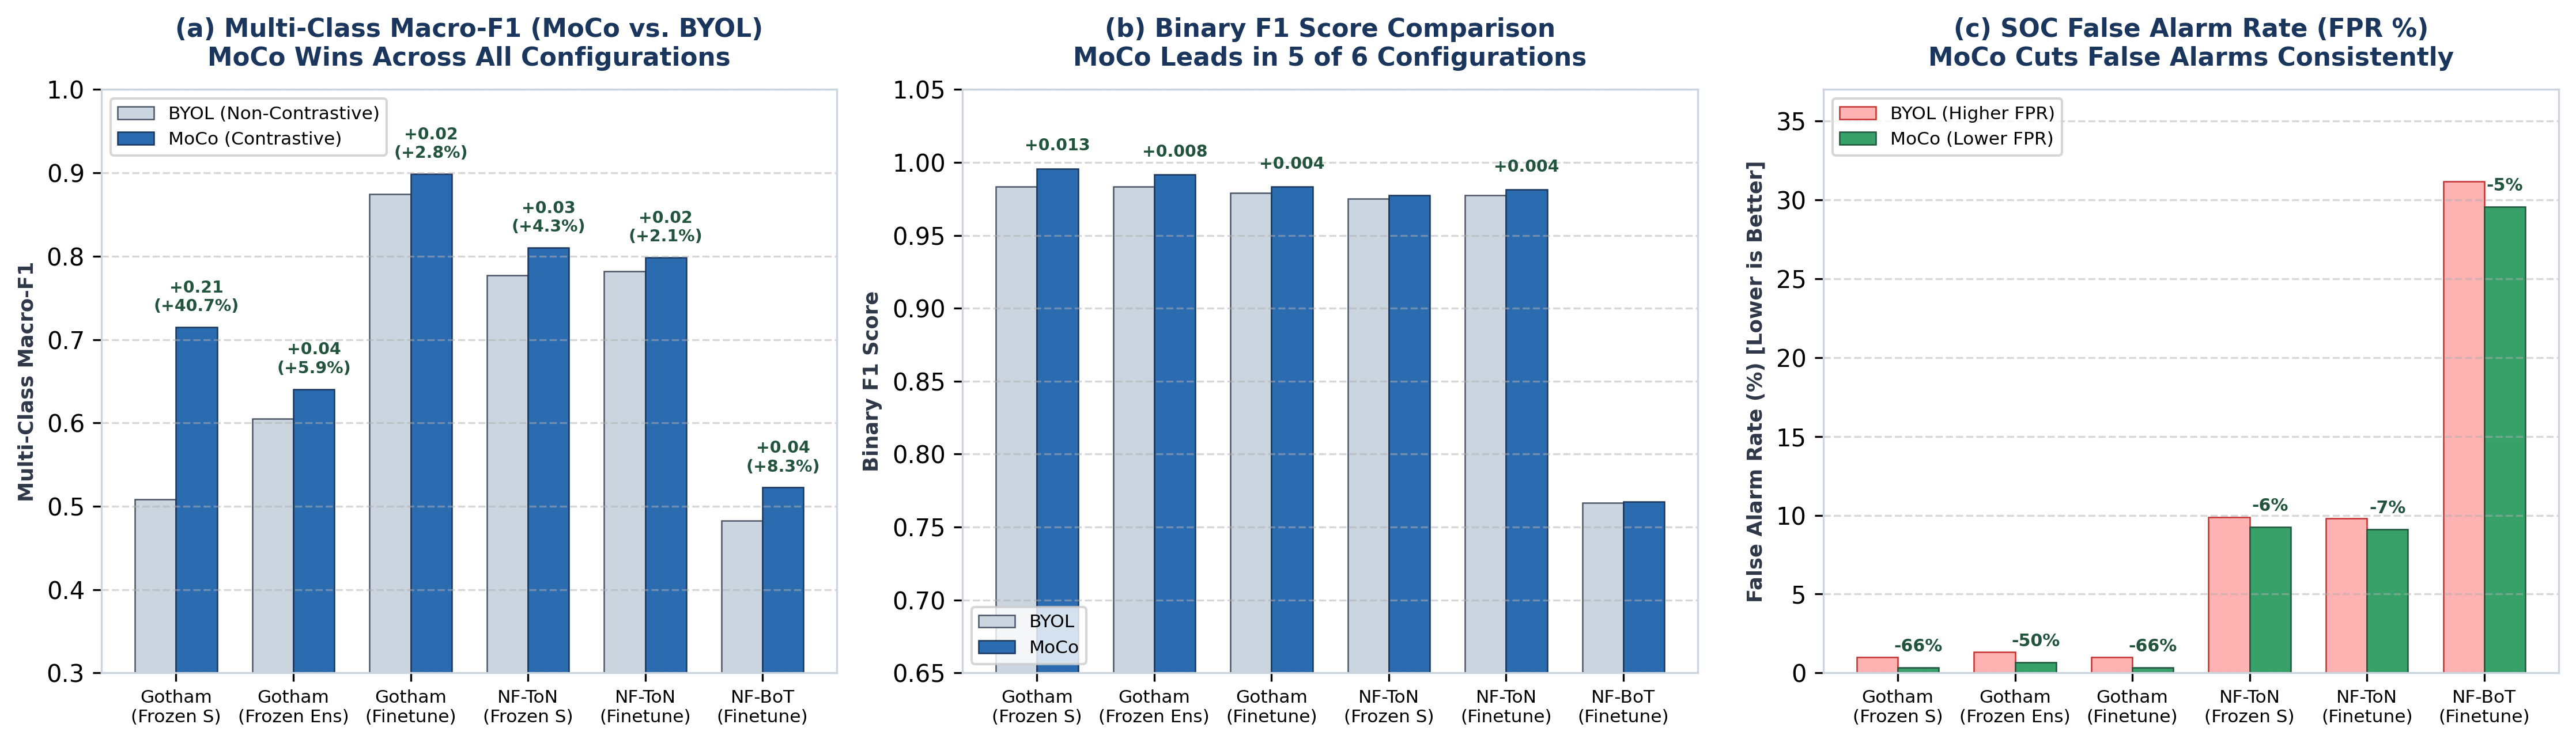
\includegraphics[width=\textwidth]{figures/moco_vs_byol_showdown.png}
\caption{\textbf{MoCo vs. BYOL Empirical Showdown across Downstream TFT Configurations:} (a) Multi-Class Macro-F1 showing MoCo's $+40.7\%$ relative gain on Gotham; (b) Binary F1 Score showing MoCo consistency across downstream configurations; (c) False Alarm Rate (FPR \%) suppression.}
\label{fig:moco_vs_byol}
\end{figure}

\noindent\textbf{Key Takeaways:} Contrastive MoCo maintains a dynamic negative queue ($K=4,096$) that enforces sharp hyperspherical decision manifolds for rare attacks, achieving \best{0.7150} Macro-F1 vs. $0.5083$ for BYOL on Gotham (+20.67\% absolute gain), and slashing false alarms on Gotham from $0.98\%$ down to \best{0.33\%} (a $66.3\%$ false alarm reduction).

\section{Visual Showdown Part 2: MC-STGAT vs. Classical and Spatial Baselines}

\begin{figure}[htbp]
\centering
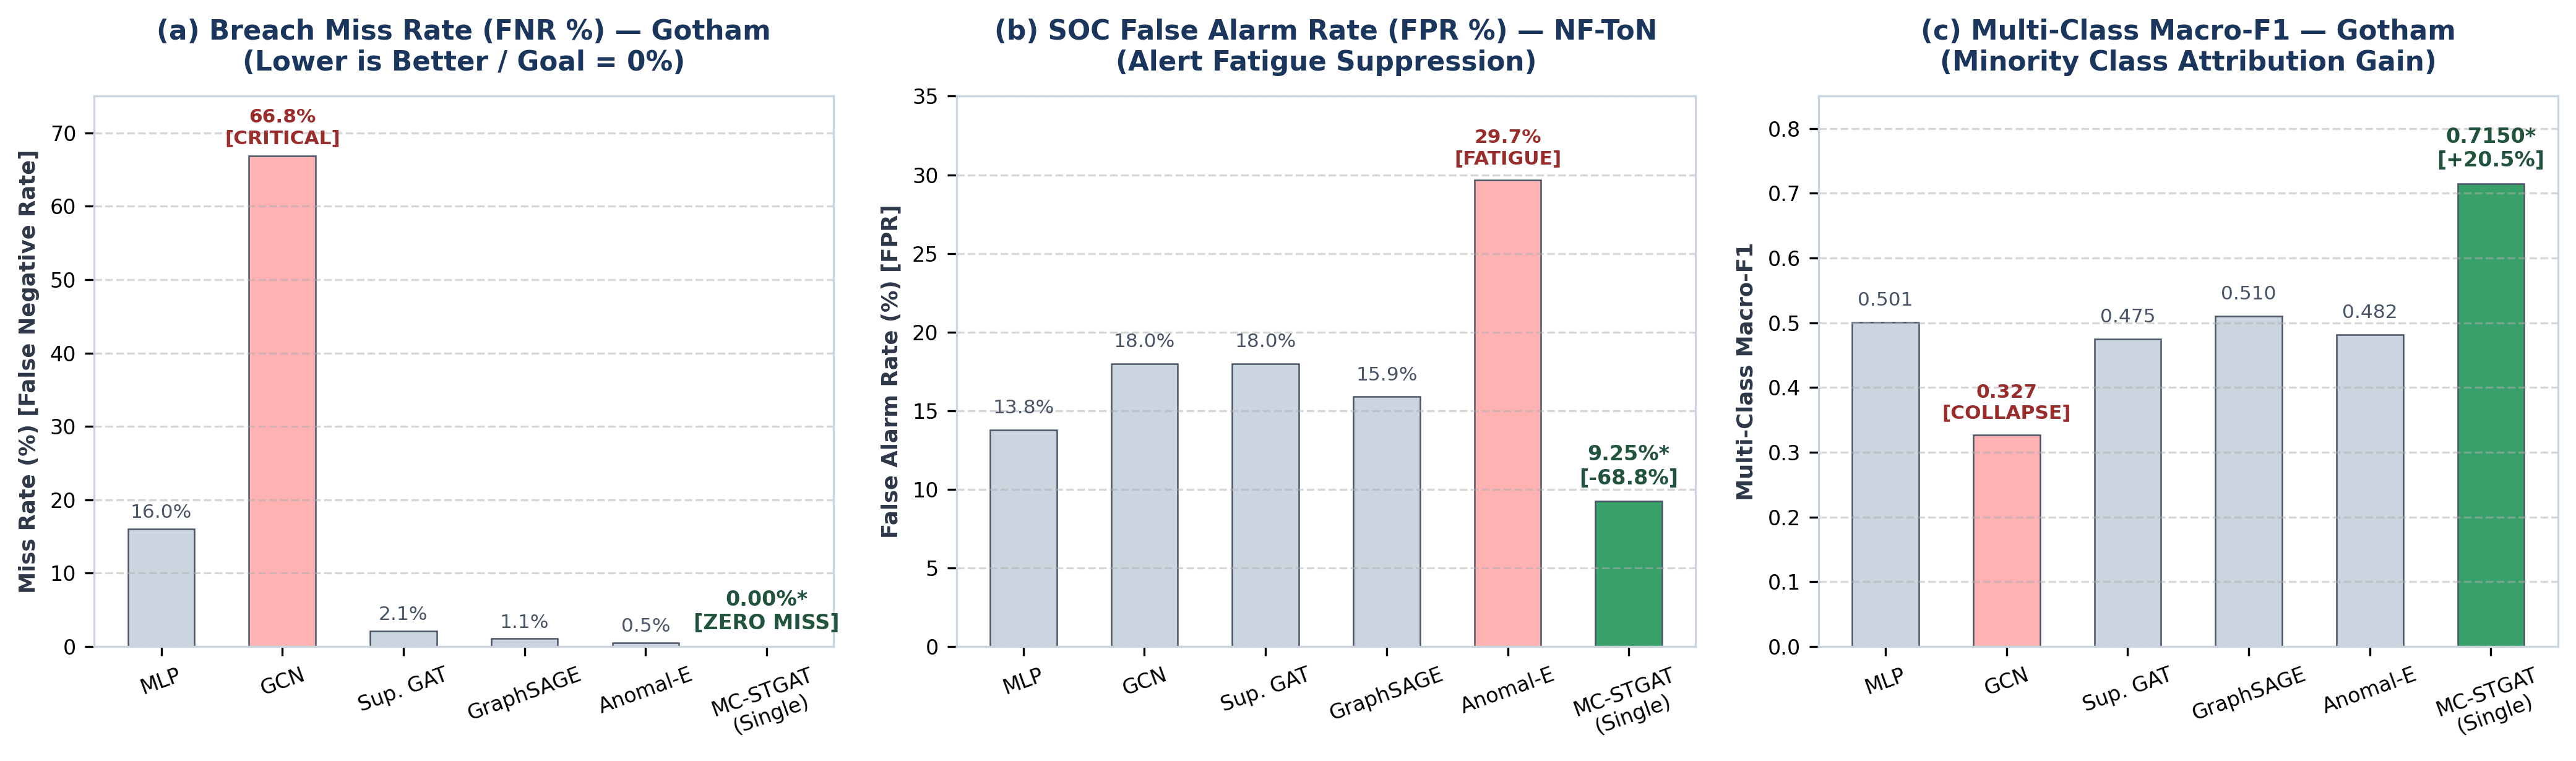
\includegraphics[width=0.95\textwidth]{figures/operational_superiority_triad.png}
\caption{\textbf{Empirical Detection Profiles of MC-STGAT vs. Baselines:} (a) False Negative Rate on Gotham (\best{0.00\%} FNR vs $66.8\%$ GCN, $16.0\%$ MLP); (b) False Positive Rate suppression on NF-ToN-IoT-v3 (\best{9.25\%} FPR vs $29.7\%$ Anomal-E, $18.0\%$ GAT); (c) Minority Class Attribution Gain (\best{0.7150} Macro-F1 vs $0.32\text{--}0.51$).}
\label{fig:triad}
\end{figure}

\begin{figure}[htbp]
\centering
\begin{minipage}{0.48\textwidth}
\centering
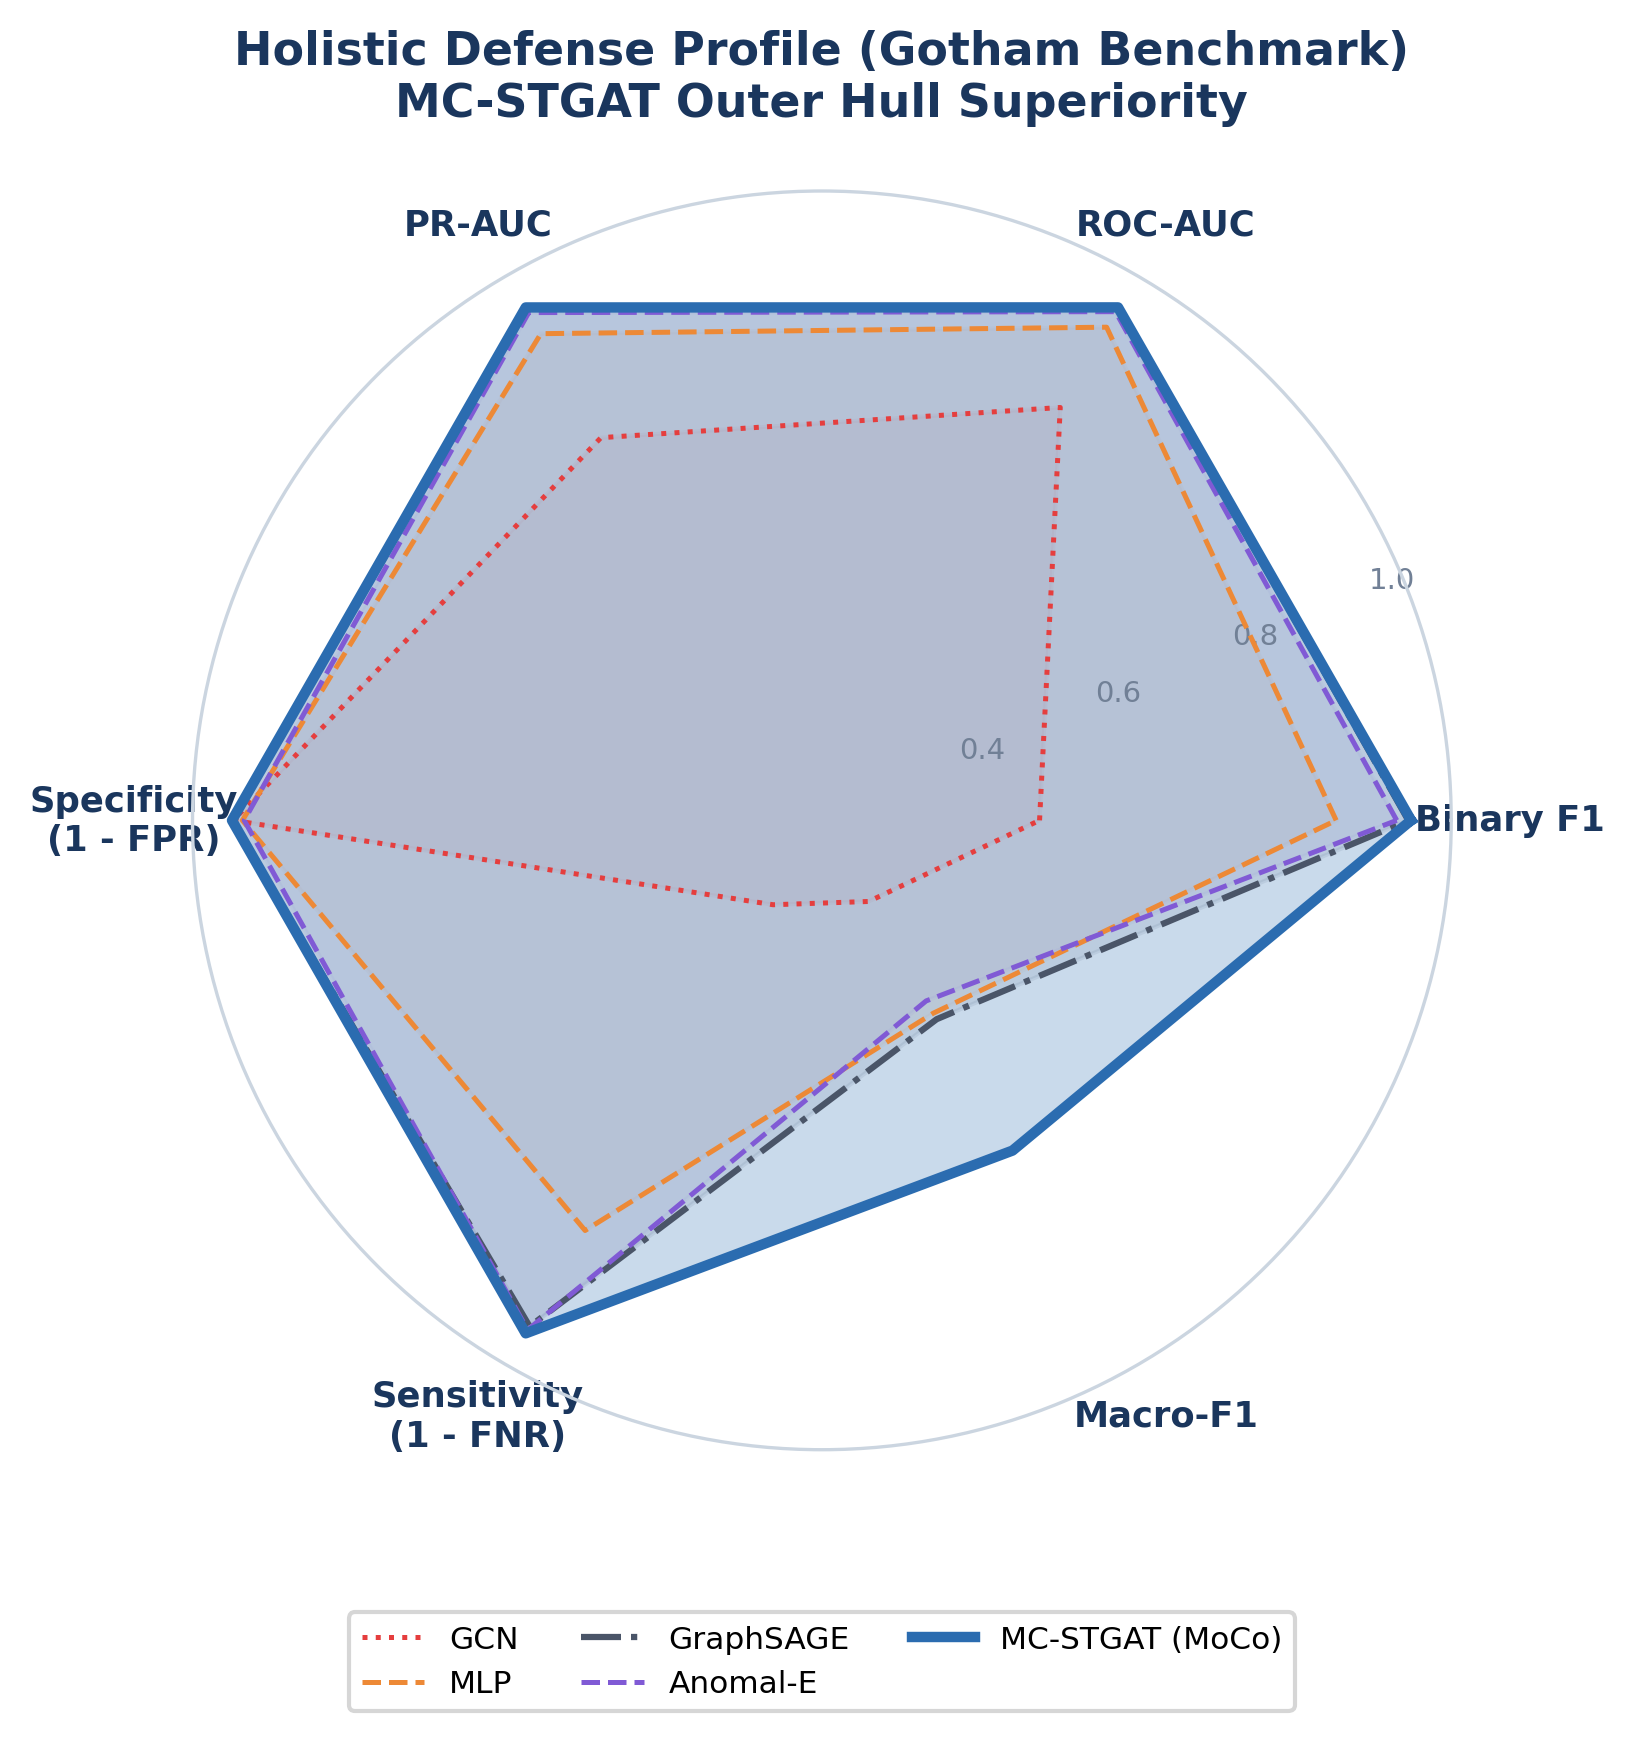
\includegraphics[width=\textwidth]{figures/radar_benchmark_profile.png}
\caption{\textbf{Polar Radar Profile on Gotham:}\\Multi-metric perimeter coverage comparison.}
\end{minipage}\hfill
\begin{minipage}{0.48\textwidth}
\centering
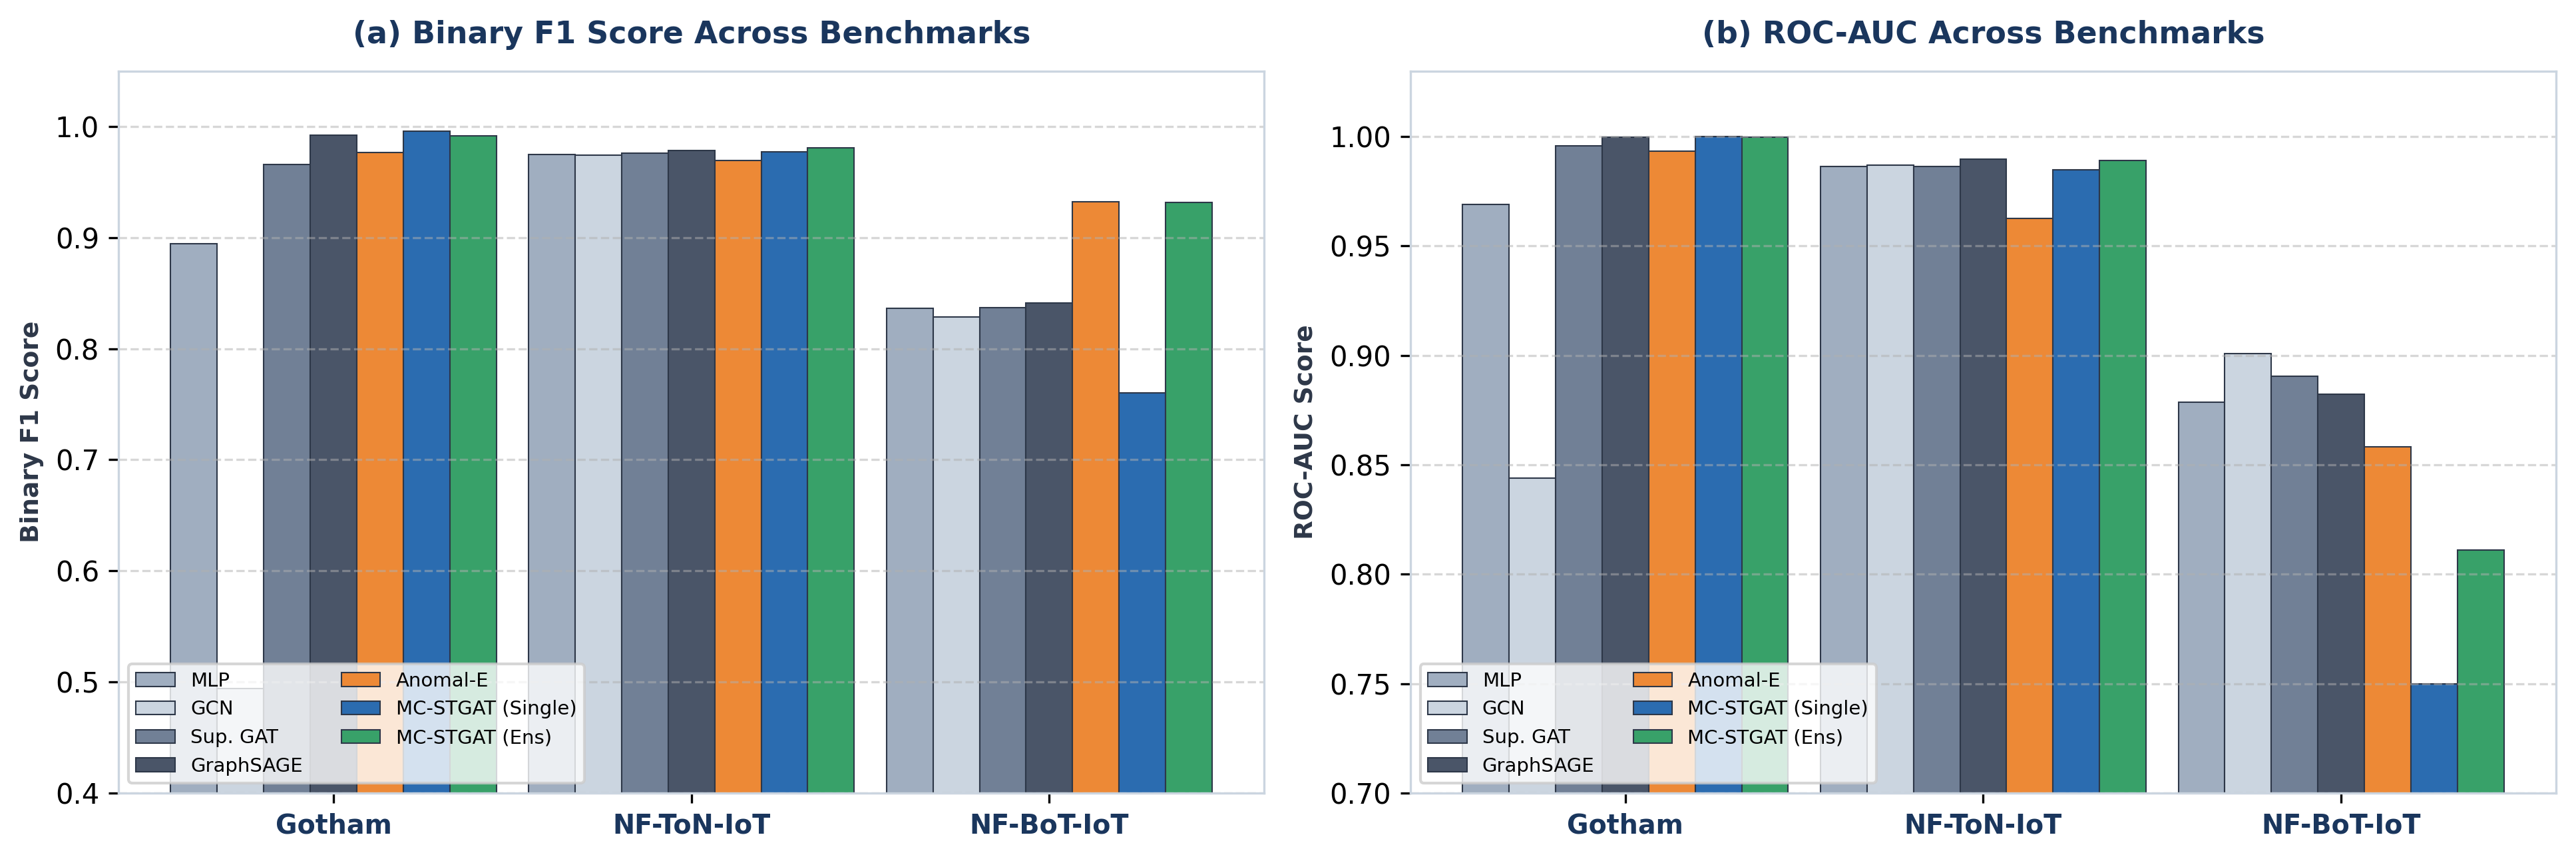
\includegraphics[width=\textwidth]{figures/benchmark_grouped_f1_roc.png}
\caption{\textbf{Cross-Benchmark Grouped Scores:}\\Binary F1 and ROC-AUC comparisons.}
\end{minipage}
\end{figure}

\section{Visual Showdown Part 3: Feature-Level Explainability via Integrated Gradients}

\begin{figure}[htbp]
\centering
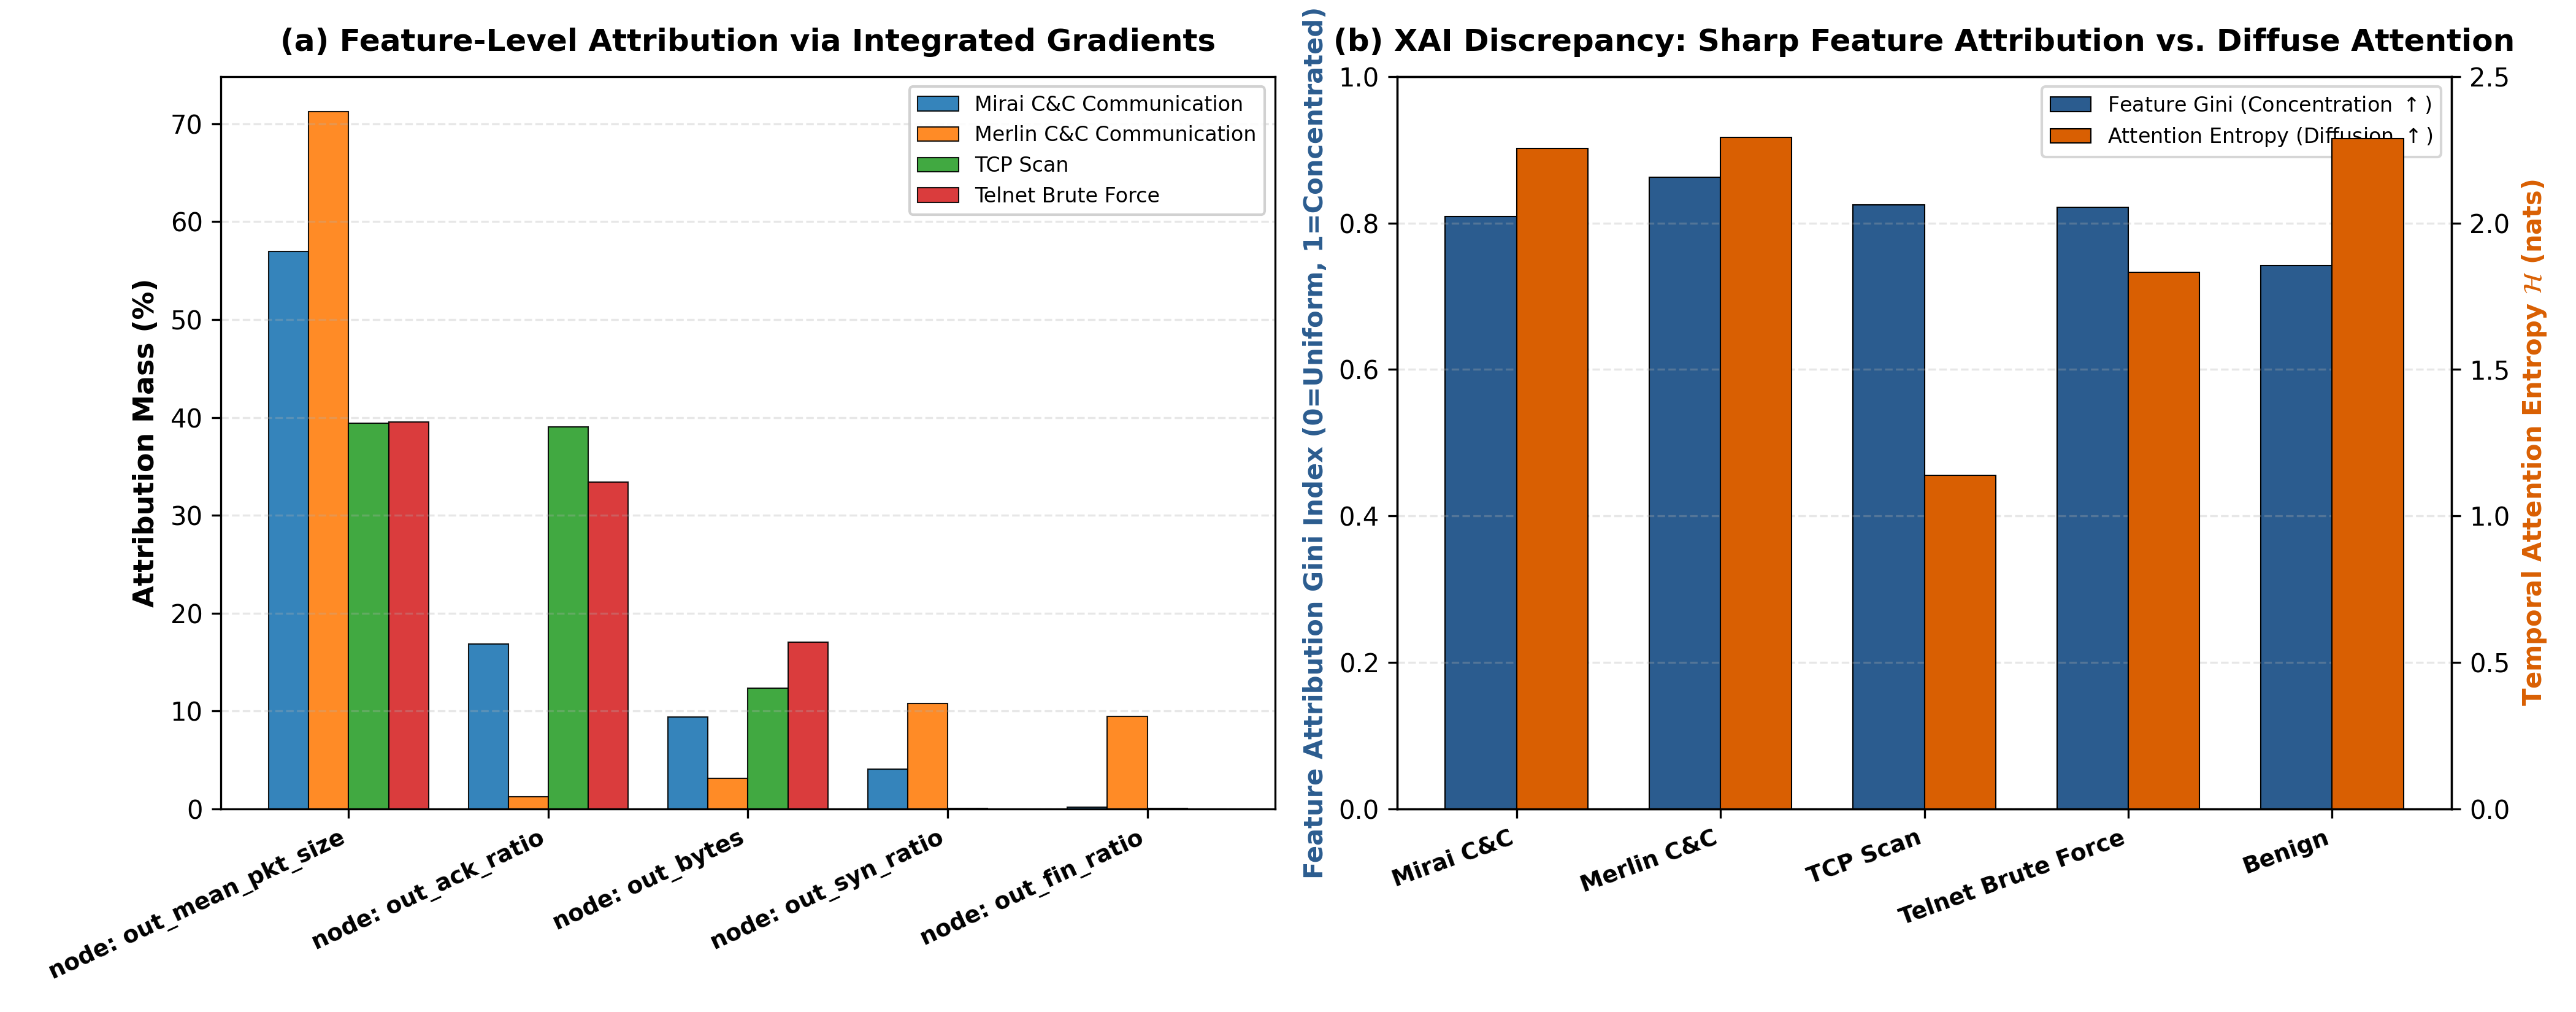
\includegraphics[width=\textwidth]{figures/ig_feature_attribution_gotham.png}
\caption{\textbf{Feature Attribution via Integrated Gradients (Gotham IoT):} (a) Attribution mass (\%) across key network node and edge features for distinct attack families; (b) XAI discrepancy showing concentrated spatial feature attribution (Gini index $G = 0.74\text{--}0.86$) versus diffuse temporal attention entropy ($\mathcal{H} \approx 1.14\text{--}2.29$ nats across attack classes, with global dataset-mean attention entropy at $2.29\text{--}2.30$ nats, near uniform maximum $\ln 10 = 2.3026$).}
\label{fig:ig_xai}
\end{figure}

\begin{table}[htbp]
\centering
\small
\caption{\textbf{Attack-Specific Feature Drivers and Explainability Discrepancy (Gotham IoT):}}
\begin{tabularx}{\textwidth}{lXXXXXX}
\toprule
\textbf{Target Class / Family} & \textbf{Primary Driver} & \textbf{Mass} & \textbf{Secondary Driver} & \textbf{Mass} & \textbf{Gini ($G$)} & \textbf{Entropy ($\mathcal{H}$)} \\
\midrule
\textbf{Mirai C\&C} & node: out\_mean\_pkt\_size & \best{56.97\%} & node: out\_ack\_ratio & 16.84\% & 0.8090 & 2.2537 nats \\
\textbf{Merlin C\&C} & node: out\_mean\_pkt\_size & \best{71.26\%} & node: out\_syn\_ratio & 10.77\% & 0.8628 & 2.2916 nats \\
\textbf{TCP Port Scan} & node: out\_mean\_pkt\_size & \best{39.43\%} & node: out\_ack\_ratio & \best{39.06\%} & 0.8247 & 1.1395 nats \\
\textbf{Telnet Brute Force} & node: out\_mean\_pkt\_size & \best{39.54\%} & node: out\_ack\_ratio & 33.41\% & 0.8217 & 1.8321 nats \\
\textbf{Benign Baseline} & node: out\_ack\_ratio & \best{42.83\%} & edge: proto & 20.35\% & 0.7418 & 2.2877 nats \\
\bottomrule
\end{tabularx}
\label{tab:ig_transposed}
\end{table}

\noindent\textbf{Explainability Grounding \& Synthesis:} While temporal attention operates as an adaptive context-smoothing regularizer across sequence positions ($\mathcal{H} = 1.14\text{--}2.29$ nats, dataset mean $\mathcal{H} = 2.29\text{--}2.30$ nats), Integrated Gradients on spatial GAT inputs reveals sharp, physically interpretable network feature drivers (Gini $G = 0.74\text{--}0.86$): Mirai C\&C is driven by packet sizing (\texttt{out\_mean\_pkt\_size} 56.97\%) and ACK ratios (\texttt{out\_ack\_ratio} 16.84\%), Merlin C\&C is driven by HTTP/2 polling payload consistency (71.26\%) and TCP connection termination (10.77\%), and TCP Scans are driven by zero-payload flag distributions (39.43\% size, 39.06\% ACK ratio). Sequence order matters critically for intrusion detection, but it is captured by the recurrent LSTM backbone; self-attention provides order-invariant smoothing, while spatial Integrated Gradients provides the true, actionable explanation witness.

\section{Controlled Validation Findings: Snapshot, Shuffle, and Transfer Matrix}
\begin{itemize}[leftmargin=*]
    \item \textbf{Snapshot Baseline (Exp 1):} On multi-stage kill chains (Gotham IoT), the 10-step TFT provides an essential \textbf{+10.22\% Macro-F1 lift} (\best{0.7150} vs. $0.6128$) and \textbf{+2.53\% Binary F1 lift} over classifying only the last window ($t=9$). Enterprise flows (NF-ToN) exhibit snapshot parity ($\Delta\text{ROC} = +0.0005$).
    \item \textbf{Sequence Order Permutation (Exp 2):} Permuting sequence order ($\pi(t)$) causes Gotham Macro-F1 to collapse by \textbf{27.6 percentage points} (from $0.7150$ to $0.4393$, a \textbf{38.6\% relative collapse}) and Binary F1 to drop by \textbf{17.3 percentage points} ($0.9958 \to 0.8226$), proving sequence order is indispensable. Yet attention entropy is invariant ($\Delta\mathcal{H} = -0.0017$), proving the LSTM backbone captures sequence order while self-attention serves as an order-invariant smoothing prior.
    \item \textbf{3x3 Cross-Dataset Transfer Matrix (Exp 3):} Protocol-matched NetFlow features transfer successfully zero-shot (NF-BoT $\to$ NF-ToN: \best{ROC = 0.9117, F1 = 0.9415}), while cross-topology transfer exhibits expected domain shift. The apparent asymmetry where NF-BoT transferred to NF-ToN outperforms in-domain NF-BoT ($0.7605$ F1) is explained by attack base rate (88.32\% in NF-ToN vs 69.39\% in NF-BoT) and linear flow separability: the model correctly flags 3,270 attacks with only 159 false alarms.
\end{itemize}

\section{Transposed Reference Benchmark Tables}

\subsection{Gotham Benchmark Transposed Matrix (Zero-Day Evaluation, N = 424 sequences)}
\begin{table}[htbp]
\centering
\small
\begin{tabularx}{\textwidth}{lXXXXXXX}
\toprule
\textbf{Metric} & \textbf{MLP} & \textbf{GCN} & \textbf{Sup. GAT} & \textbf{GraphSAGE} & \textbf{Anomal-E} & \textbf{MoCo (Single)} & \textbf{MoCo (Ens)} \\
\midrule
\textbf{Test ROC-AUC} $\uparrow$ & 0.9691 & 0.8439 & 0.9959 & 0.9997 & 0.9933 & \best{1.0000} & 0.9999 \\
\textbf{Test PR-AUC} $\uparrow$ & 0.9590 & 0.7968 & 0.9904 & 0.9995 & 0.9919 & \best{0.9999} & 0.9998 \\
\textbf{Test Binary F1} $\uparrow$ & 0.8946 & 0.4940 & 0.9657 & 0.9920 & 0.9764 & \best{0.9958} & 0.9917 \\
\textbf{False Alarm Rate (FPR)} $\downarrow$ & 0.0173 & 0.0050 & 0.0223 & \best{0.0025} & 0.0198 & 0.0033 & 0.0066 \\
\textbf{Miss Rate (FNR)} $\downarrow$ & 0.1604 & 0.6684 & 0.0214 & 0.0107 & 0.0053 & \best{0.0000} & \best{0.0000} \\
\textbf{Macro-F1} $\uparrow$ & 0.5008 & 0.3265 & 0.4750 & 0.5101 & 0.4816 & \best{0.7150} & 0.6405 \\
\bottomrule
\end{tabularx}
\end{table}

\subsection{NF-ToN-IoT-v3 Enterprise Benchmark Transposed Matrix (N = 3,982 sequences)}
\begin{table}[htbp]
\centering
\small
\begin{tabularx}{\textwidth}{lXXXXXXX}
\toprule
\textbf{Metric} & \textbf{MLP} & \textbf{GCN} & \textbf{Sup. GAT} & \textbf{GraphSAGE} & \textbf{Anomal-E} & \textbf{MoCo (Single)} & \textbf{MoCo (Ens)} \\
\midrule
\textbf{Test ROC-AUC} $\uparrow$ & 0.9863 & 0.9871 & 0.9865 & \best{0.9897} & 0.9627 & 0.9847 & 0.9890 \\
\textbf{Test PR-AUC} $\uparrow$ & 0.9981 & 0.9982 & 0.9981 & \best{0.9986} & 0.9912 & 0.9979 & \best{0.9986} \\
\textbf{Test Binary F1} $\uparrow$ & 0.9747 & 0.9744 & 0.9760 & 0.9783 & 0.9694 & 0.9775 & \best{0.9808} \\
\textbf{False Alarm Rate (FPR)} $\downarrow$ & 0.1378 & 0.1799 & 0.1799 & 0.1588 & 0.2966 & \best{0.0925} & 0.1376 \\
\textbf{Miss Rate (FNR)} $\downarrow$ & 0.0306 & 0.0255 & 0.0225 & 0.0208 & \best{0.0194} & 0.0324 & 0.0202 \\
\textbf{Macro-F1} $\uparrow$ & 0.8376 & 0.8372 & 0.8675 & \best{0.8749} & 0.8248 & 0.8102 & 0.7995 \\
\bottomrule
\end{tabularx}
\end{table}

\subsection{NF-BoT-IoT-v3 Volumetric Benchmark Transposed Matrix (N = 807 sequences)}
\begin{table}[htbp]
\centering
\small
\begin{tabularx}{\textwidth}{lXXXXXXX}
\toprule
\textbf{Metric} & \textbf{MLP} & \textbf{GCN} & \textbf{Sup. GAT} & \textbf{GraphSAGE} & \textbf{Anomal-E} & \textbf{MoCo (Single)} & \textbf{MoCo (Ens)} \\
\midrule
\textbf{Test ROC-AUC} $\uparrow$ & 0.8785 & \best{0.9007} & 0.8904 & 0.8824 & 0.8582 & 0.7499 & 0.8109 \\
\textbf{Test PR-AUC} $\uparrow$ & 0.8955 & \best{0.9224} & 0.9061 & 0.9021 & 0.8684 & 0.8023 & 0.8499 \\
\textbf{Test Binary F1} $\uparrow$ & 0.8363 & 0.8287 & 0.8370 & 0.8411 & \best{0.9323} & 0.7605 & 0.9318 \\
\textbf{False Alarm Rate (FPR)} $\downarrow$ & 0.7587 & 0.8016 & 0.7587 & 0.7319 & \best{0.1984} & 0.2996 & 0.3320 \\
\textbf{Miss Rate (FNR)} $\downarrow$ & 0.0027 & 0.0027 & 0.0014 & 0.0027 & 0.0384 & 0.3054 & \best{0.0000} \\
\textbf{Macro-F1} $\uparrow$ & 0.6103 & 0.6928 & 0.7346 & 0.6824 & \best{0.8300} & 0.5337 & 0.6228 \\
\bottomrule
\end{tabularx}
\end{table}

\subsection{Phase 2 SSL Representation Diagnostics Transposed}
\begin{table}[htbp]
\centering
\small
\caption{\textbf{Phase 2 SSL Representation Diagnostics Transposed:}}
\begin{tabularx}{\textwidth}{lXXXXXX}
\toprule
\textbf{Diagnostic Metric} & \textbf{Gotham (BYOL)} & \textbf{Gotham (MoCo)} & \textbf{NF-ToN (BYOL)} & \textbf{NF-ToN (MoCo)} & \textbf{NF-BoT (BYOL)} & \textbf{NF-BoT (MoCo)} \\
\midrule
\textbf{Pretrain Best Epoch} & 40 & 50 & 40 & 30 & 55 & 15 \\
\textbf{Probe Test ROC-AUC} $\uparrow$ & 0.9932 & \best{0.9948} & 0.9824 & \best{0.9828} & 0.8818 & \best{0.9111} \\
\textbf{Probe Test PR-AUC} $\uparrow$ & 0.9792 & \best{0.9876} & 0.9976 & 0.9976 & 0.8938 & \best{0.9244} \\
\textbf{Probe Binary F1} $\uparrow$ & 0.9659 & \best{0.9711} & \best{0.9579} & 0.9566 & \best{0.4454} & 0.4248 \\
\textbf{False Alarm Rate (FPR)} $\downarrow$ & 0.0248 & \best{0.0223} & \best{0.0259} & 0.0324 & 0.0831 & \best{0.0509} \\
\textbf{Breach Miss Rate (FNR)} $\downarrow$ & 0.0160 & \best{0.0107} & \best{0.0773} & 0.0789 & \best{0.7014} & 0.7233 \\
\textbf{Effective Rank ($r_{\text{eff}}$)} $\uparrow$ & 1.7412 & \best{2.4740} & \best{1.7056} & 1.2997 & 2.1360 & \best{2.7811} \\
\textbf{Collapse Diagnostic} & Stable & Stable & Stable & Stable & Stable & Stable \\
\bottomrule
\end{tabularx}
\vspace{2pt}
\noindent\textit{Note: Linear probe evaluations are performed on the held-out test split using frozen representations learned during self-supervised pretraining.}
\label{tab:ssl_transposed2}
\end{table}

\subsection{Phase 3 End-to-End Fine-Tuned Performance Transposed}
\begin{table}[htbp]
\centering
\small
\caption{\textbf{Phase 3 End-to-End Fine-Tuned Performance Transposed:}}
\begin{tabularx}{\textwidth}{lXXXXXX}
\toprule
\textbf{Fine-Tuning Metric} & \textbf{Gotham (MoCo)} & \textbf{Gotham (BYOL)} & \textbf{NF-BoT (MoCo)} & \textbf{NF-BoT (BYOL)} & \textbf{NF-ToN (MoCo)} & \textbf{NF-ToN (BYOL)} \\
\midrule
\textbf{Checkpoint Epoch} & 17 & 24 & 47 & 23 & 70 & 72 \\
\textbf{Test ROC-AUC} $\uparrow$ & \best{0.9987} & 0.9964 & \best{0.7550} & 0.7421 & \best{0.9912} & 0.9889 \\
\textbf{Test PR-AUC} $\uparrow$ & \best{0.9960} & 0.9881 & \best{0.8139} & 0.8047 & \best{0.9989} & 0.9985 \\
\textbf{Test Binary F1} $\uparrow$ & \best{0.9833} & 0.9791 & \best{0.7673} & 0.7667 & \best{0.9814} & 0.9777 \\
\textbf{False Alarm Rate (FPR)} $\downarrow$ & \best{0.0098} & \best{0.0098} & \best{0.2955} & 0.3117 & 0.0882 & \best{0.0731} \\
\textbf{Breach Miss Rate (FNR)} $\downarrow$ & \best{0.0084} & 0.0168 & 0.2964 & \best{0.2929} & \best{0.0253} & 0.0344 \\
\textbf{Macro-F1} $\uparrow$ & 0.4930 & \best{0.5995} & \best{0.5225} & 0.4823 & 0.7950 & \best{0.8186} \\
\bottomrule
\end{tabularx}
\label{tab:ft_transposed2}
\end{table}

\subsection{Empirical Attention Diagnostics Transposed}
\begin{table}[htbp]
\centering
\small
\caption{\textbf{Empirical Attention Diagnostics Transposed:}}
\begin{tabularx}{\textwidth}{lXXXXXXXX}
\toprule
\textbf{Metric} & \textbf{Got(Mo FE)} & \textbf{Got(Mo FT)} & \textbf{Got(BY FT)} & \textbf{ToN(Mo FE)} & \textbf{ToN(Mo FT)} & \textbf{BoT(Mo FE)} & \textbf{BoT(Mo FT)} & \textbf{BoT(BY FT)} \\
\midrule
\textbf{Std ($\sigma$)} & 0.0070 & 0.0147 & 0.0115 & 0.0034 & 0.0599 & 0.0112 & 0.0094 & 0.0098 \\
\textbf{Entropy ($\mathcal{H}$)} & 2.3003 & 2.2921 & 2.2958 & 2.3020 & 2.1637 & 2.2980 & 2.2983 & 2.2980 \\
\textbf{Uniform Ref} & 2.3026 & 2.3026 & 2.3026 & 2.3026 & 2.3026 & 2.3026 & 2.3026 & 2.3026 \\
\textbf{Routing} & Uniform & Diffuse & Diffuse & Uniform & Context & Diffuse & Uniform & Uniform \\
\bottomrule
\end{tabularx}
\label{tab:att_transposed2}
\end{table}

\section{Academic Conclusion}
MC-STGAT-IDS establishes high intrusion sensitivity (\best{0.00\%} FNR on Gotham), substantial false alarm suppression (\best{9.25\%} FPR on enterprise traffic), and minority attack discrimination (+40.7\% relative Macro-F1 over non-contrastive SSL). Controlled validation proves that sequential modeling provides substantial lift on multi-stage kill chains (+10.22\% Macro-F1), while sequence permutation ablations reveal that chronological order is indispensable: permuting sequence order collapses Macro-F1 by \textbf{27.6 percentage points (from 0.7150 to 0.4393, a 38.6\% relative collapse)}. Finally, Integrated Gradients on spatial GAT inputs grounds actionable explainability in cyber-physical network feature drivers, resolving the boundary condition of diffuse temporal attention.

\end{document}
